% ============================================================================
%  Getting more from every experiment
%  Optimal design, the OWEA algorithm, and the OWEAdesign package
%
%  Compile (recommended):   xelatex owea_slides.tex   (run twice)
%  Also works with:         pdflatex owea_slides.tex  (run twice)
%  Requires the metropolis beamer theme (in TeX Live) and the img/ folder.
% ============================================================================
\documentclass[aspectratio=169,10pt]{beamer}
\usetheme[progressbar=frametitle,numbering=fraction,block=fill]{metropolis}

\usepackage{amsmath,amssymb,bm}
\usepackage{booktabs,multicol}
\usepackage{tikz}
\usetikzlibrary{arrows.meta,positioning,calc,shapes.misc}
\usepackage{graphicx}
\graphicspath{{img/}}
\usepackage{iftex}
\ifXeTeX
  \usepackage{fontspec}
  % Lato (OFL) ships in fonts/ so the deck looks the same on every machine.
  \setsansfont[Path=fonts/, Extension=.ttf, UprightFont=lato-v16-latin-regular,
               BoldFont=lato-v16-latin-700, ItalicFont=lato-v16-latin-300italic,
               BoldItalicFont=lato-v16-latin-700]{Lato}
  \setmonofont[Path=fonts/, Extension=.ttf, Scale=0.85]{DejaVuSansMono}
\else
  \usepackage[T1]{fontenc}
  \usepackage[scaled]{helvet}
\fi
\usepackage{listings}

% ---------------------------------------------------------------- colours
\definecolor{navy}{HTML}{1F3B5C}
\definecolor{brick}{HTML}{C0392B}
\definecolor{sky}{HTML}{1F77B4}
\definecolor{ink}{HTML}{23373B}
\definecolor{paper}{HTML}{FAFAFA}
\setbeamercolor{normal text}{fg=ink,bg=white}
\setbeamercolor{frametitle}{bg=navy,fg=white}
\setbeamercolor{progress bar}{fg=brick,bg=navy!25}
\setbeamercolor{alerted text}{fg=brick}
\setbeamercolor{example text}{fg=navy}
\setbeamercolor{block title}{bg=navy!12,fg=navy}
\setbeamercolor{block body}{bg=navy!5}
\setbeamercolor{block title alerted}{bg=brick!12,fg=brick}
\setbeamercolor{block body alerted}{bg=brick!5}
\setbeamertemplate{section in toc}[sections numbered]
\metroset{sectionpage=progressbar}

\newcommand{\hl}[1]{\textcolor{brick}{\textbf{#1}}}
\newcommand{\key}[1]{\textcolor{navy}{\textbf{#1}}}
\newcommand{\Var}{\operatorname{Var}}
\newcommand{\tr}{\operatorname{tr}}
\newcommand{\shotsm}[1]{{\setlength{\fboxsep}{0pt}\fcolorbox{gray!45}{white}{\includegraphics[width=\dimexpr\linewidth-2\fboxrule\relax,height=0.5\textheight,keepaspectratio]{#1}}}}
\newcommand{\shot}[1]{{\setlength{\fboxsep}{0pt}\fcolorbox{gray!45}{white}{\includegraphics[width=\dimexpr\linewidth-2\fboxrule\relax,height=0.62\textheight,keepaspectratio]{#1}}}}

\lstset{language=R,basicstyle=\ttfamily\scriptsize,keywordstyle=\color{navy}\bfseries,
  commentstyle=\color{gray},stringstyle=\color{brick},showstringspaces=false,
  columns=fullflexible,keepspaces=true}

% ---------------------------------------------------------------- title
\title{Getting more from every experiment}
\subtitle{Optimal design, the OWEA algorithm, and the \texttt{OWEAdesign} package}
\author{Min Yang}
\institute{University of Illinois at Chicago}
\date{}

\begin{document}

\maketitle

% ============================================================================
\begin{frame}{Two experiments}
  \begin{columns}[T]
    \begin{column}{0.5\textwidth}
      \begin{block}{Experiment A}
        Same question. Same precision.\\[2pt]
        \hl{16 measurements}. Cost: \hl{\$16}.
      \end{block}
    \end{column}
    \begin{column}{0.5\textwidth}
      \begin{block}{Experiment B}
        Same question. Same precision.\\[2pt]
        \key{4 measurements}. Cost: \key{\$4}.
      \end{block}
    \end{column}
  \end{columns}
  \vspace{1.2em}
  \centering
  \Large The only difference: \alert{how the measurements were arranged.}

  \vspace{1em}
  \normalsize
  This talk is about how to find Experiment~B---by hand for small problems,
  and with a click for everything else.
\end{frame}

\begin{frame}{Roadmap}
  \tableofcontents
\end{frame}

% ============================================================================
\section{What optimal design does}

\begin{frame}{Statistics has two halves}
  \begin{columns}[T]
    \begin{column}{0.48\textwidth}
      \begin{block}{Analysis (the famous half)}
        Given the data, what can we conclude?\\
        Estimates, confidence intervals, tests, models.
      \end{block}
    \end{column}
    \begin{column}{0.48\textwidth}
      \begin{alertblock}{Design (the quiet half)}
        Before any data exist: \emph{which} measurements should we take, and \emph{how many} of each?
      \end{alertblock}
    \end{column}
  \end{columns}
  \vspace{1em}
  \begin{itemize}
    \item Analysis can only squeeze out the information the data contain.
    \item \key{Design decides how much information there is to squeeze.}
    \item An \key{optimal design} gives the most precise answer for a fixed budget---or,
          equivalently, reaches a target precision with the smallest budget.
  \end{itemize}
\end{frame}

\begin{frame}{What we will do today}
  \begin{enumerate}
    \item See the idea on a \key{balance scale} with four pieces of fruit \hfill (no formulas)
    \item Write the same idea down in general \hfill (a few formulas, gently)
    \item Meet \key{OWEA}, the algorithm that finds optimal designs \hfill (one picture)
    \item Use the \key{\texttt{OWEAdesign} web app} to design a real experiment \hfill (no code)
  \end{enumerate}
  \vspace{1em}
  \begin{center}
    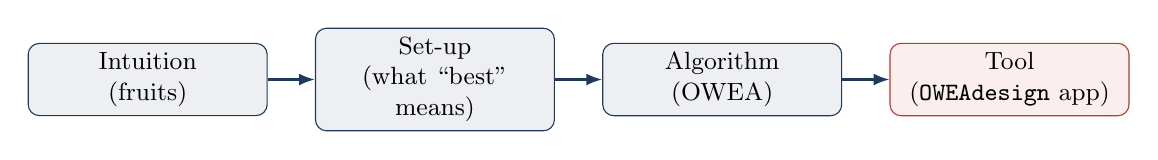
\begin{tikzpicture}[node distance=6mm, every node/.style={font=\small}]
      \node[draw=navy,rounded corners,fill=navy!8,minimum height=9mm,text width=28mm,align=center] (a) {Intuition\\ (fruits)};
      \node[draw=navy,rounded corners,fill=navy!8,minimum height=9mm,text width=28mm,align=center,right=of a] (b) {Set-up\\ (what ``best'' means)};
      \node[draw=navy,rounded corners,fill=navy!8,minimum height=9mm,text width=28mm,align=center,right=of b] (c) {Algorithm\\ (OWEA)};
      \node[draw=brick,rounded corners,fill=brick!8,minimum height=9mm,text width=28mm,align=center,right=of c] (d) {Tool\\ (\texttt{OWEAdesign} app)};
      \draw[-{Latex[length=2mm]},navy,thick] (a) -- (b);
      \draw[-{Latex[length=2mm]},navy,thick] (b) -- (c);
      \draw[-{Latex[length=2mm]},navy,thick] (c) -- (d);
    \end{tikzpicture}
  \end{center}
\end{frame}

% ============================================================================
\section{A balance-scale story}

\begin{frame}{The problem}
  \begin{columns}[c]
    \begin{column}{0.55\textwidth}
      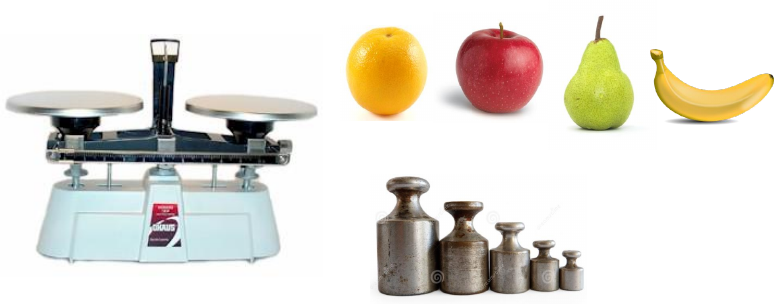
\includegraphics[width=\linewidth,height=0.7\textheight,keepaspectratio]{crop_04}
    \end{column}
    \begin{column}{0.45\textwidth}
      We want the weights of four fruits: $A$, $B$, $C$, $D$.
      \vspace{0.6em}
      \begin{itemize}
        \item We have a balance and a set of standard weights.
        \item Every weighing has a small random error $\epsilon$ with variance $\sigma^2$.
        \item \hl{Each weighing costs \$1.} We can afford four.
      \end{itemize}
      \vspace{0.6em}
      How should we spend the four weighings?
    \end{column}
  \end{columns}
  \vfill
  \begin{center}
    \small \textcolor{sky}{\textbf{An animated version of this example:}} \url{https://www.youtube.com/watch?v=5qewz8EYBzQ}
  \end{center}
\end{frame}

\begin{frame}{Design I: the obvious plan}
  \begin{columns}[c]
    \begin{column}{0.5\textwidth}
      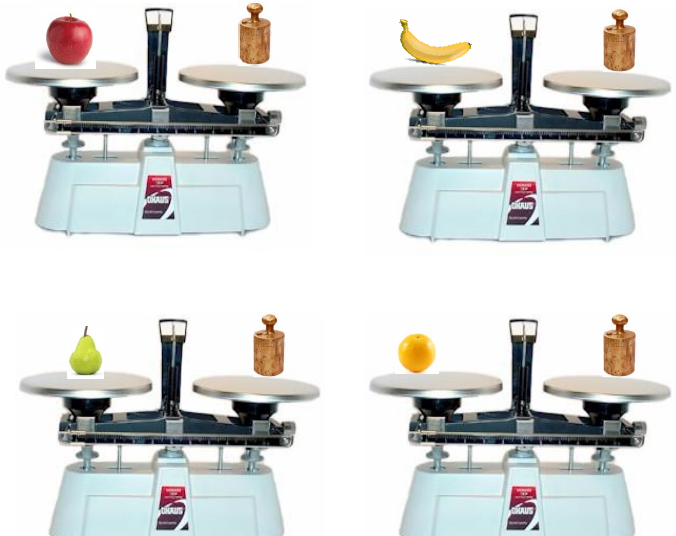
\includegraphics[width=\linewidth,height=0.7\textheight,keepaspectratio]{crop_05}
    \end{column}
    \begin{column}{0.5\textwidth}
      Weigh each fruit on its own.
      \begin{align*}
        Y_1 &= A + \epsilon_1, & Y_2 &= B + \epsilon_2,\\
        Y_3 &= C + \epsilon_3, & Y_4 &= D + \epsilon_4.
      \end{align*}
      \[
        \hat A = Y_1,\quad \hat B = Y_2,\quad \hat C = Y_3,\quad \hat D = Y_4.
      \]
      \begin{alertblock}{Precision}
        $\Var(\hat A)=\Var(\hat B)=\Var(\hat C)=\Var(\hat D)=\sigma^2$
      \end{alertblock}
    \end{column}
  \end{columns}
\end{frame}

\begin{frame}{Design II: weigh in pairs}
  \begin{columns}[c]
    \begin{column}{0.5\textwidth}
      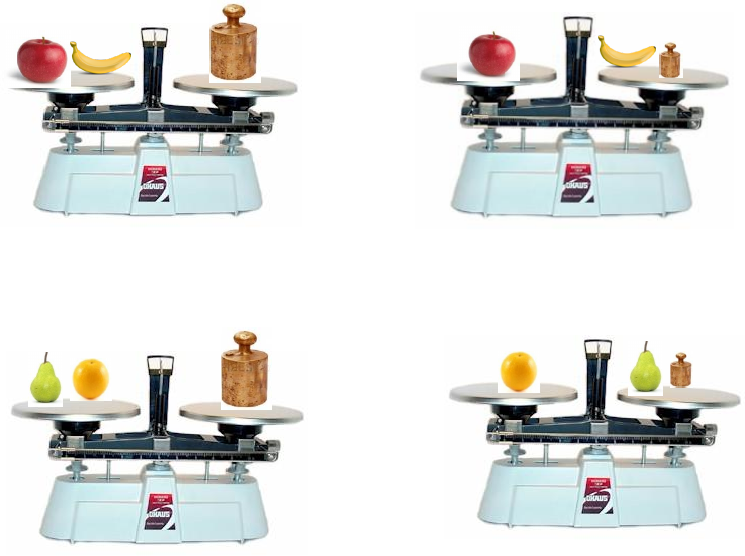
\includegraphics[width=\linewidth,height=0.7\textheight,keepaspectratio]{crop_07}
    \end{column}
    \begin{column}{0.5\textwidth}
      Two fruits per weighing: both on the left pan, or one on each pan.
      \begin{align*}
        Y_1 &= A + B + \epsilon_1, & Y_2 &= A - B + \epsilon_2,\\
        Y_3 &= C + D + \epsilon_3, & Y_4 &= C - D + \epsilon_4.
      \end{align*}
      \[
        \hat A = \tfrac{Y_1+Y_2}{2},\; \hat B = \tfrac{Y_1-Y_2}{2},\;
        \hat C = \tfrac{Y_3+Y_4}{2},\; \hat D = \tfrac{Y_3-Y_4}{2}.
      \]
      \begin{alertblock}{Precision}
        $\Var(\hat A)=\cdots=\Var(\hat D)=\sigma^2/2$
      \end{alertblock}
      Same four weighings. Half the variance.
    \end{column}
  \end{columns}
\end{frame}

\begin{frame}{Design III: every fruit, every time}
  \begin{columns}[c]
    \begin{column}{0.5\textwidth}
      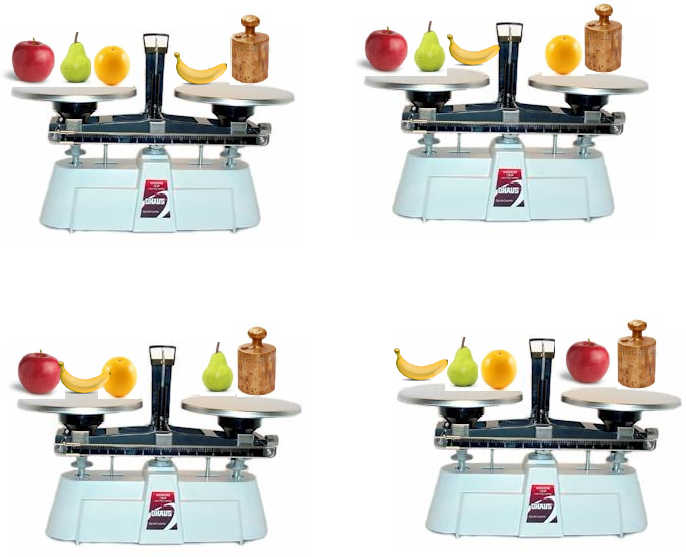
\includegraphics[width=\linewidth,height=0.7\textheight,keepaspectratio]{crop_09}
    \end{column}
    \begin{column}{0.5\textwidth}
      \small All four fruits on the scale every time: three on one pan, one on the other.
      \vspace{-0.4em}
      \begin{align*}
        Y_1 &= A + B + C - D + \epsilon_1, & Y_2 &= A + B - C + D + \epsilon_2,\\
        Y_3 &= A - B + C + D + \epsilon_3, & Y_4 &= -A + B + C + D + \epsilon_4.
      \end{align*}
      \vspace{-0.6em}
      \[
        \hat A = \tfrac{Y_1+Y_2+Y_3-Y_4}{4},\quad \hat B = \tfrac{Y_1+Y_2-Y_3+Y_4}{4},\quad\ldots
      \]
      \begin{alertblock}{Precision}
        $\Var(\hat A)=\cdots=\Var(\hat D)=\sigma^2/4$
      \end{alertblock}
    \end{column}
  \end{columns}
\end{frame}

\begin{frame}{Comparison}
  \begin{columns}[T]
    \begin{column}{0.5\textwidth}
      \centering
      \textbf{Same cost (\$4)}\\[4pt]
      \begin{tabular}{lccc}\toprule
        Design   & I          & II           & III \\ \midrule
        Variance & $\sigma^2$ & $\sigma^2/2$ & $\sigma^2/4$ \\ \bottomrule
      \end{tabular}
    \end{column}
    \begin{column}{0.5\textwidth}
      \centering
      \textbf{Same precision ($\sigma^2/4$)}\\[4pt]
      \begin{tabular}{lccc}\toprule
        Design & I    & II  & III \\ \midrule
        Cost   & \hl{\$16} & \$8 & \key{\$4} \\ \bottomrule
      \end{tabular}
    \end{column}
  \end{columns}
  \vspace{1.5em}
  \begin{block}{What the fruits teach us}
    \begin{itemize}
      \item The \emph{same} measurements, arranged differently, carry \emph{four times} the information.
      \item Design III is the optimal design for this problem. It is also the one nobody would draw on a napkin.
      \item For four fruits a clever person finds Design III by hand. \hl{For your experiment, who finds it?}
    \end{itemize}
  \end{block}
\end{frame}

% ============================================================================
\section{The general set-up}

\begin{frame}{From fruits to formulas}
  Each weighing is a row of a matrix $X$ with entries $1$, $0$ or $-1$ (left pan, absent, right pan):
  \[
    Y = X\beta + \epsilon,\qquad \beta=(A,B,C,D)',\qquad
    \hat\beta = (X'X)^{-1}X'Y,\qquad \Var(\hat\beta) = \sigma^2\,(X'X)^{-1}.
  \]
  \vspace{-0.5em}
  \[
    X_{I} = \begin{pmatrix} 1&0&0&0\\0&1&0&0\\0&0&1&0\\0&0&0&1\end{pmatrix},\quad
    X_{II} = \begin{pmatrix} 1&1&0&0\\1&-1&0&0\\0&0&1&1\\0&0&1&-1\end{pmatrix},\quad
    X_{III} = \begin{pmatrix} 1&1&1&-1\\1&1&-1&1\\1&-1&1&1\\-1&1&1&1\end{pmatrix}
  \]
  \[
    (X_I'X_I)^{-1} = I,\qquad (X_{II}'X_{II})^{-1} = \tfrac12 I,\qquad (X_{III}'X_{III})^{-1} = \tfrac14 I.
  \]
  \begin{alertblock}{The design problem in one sentence}
    Choose the rows of $X$ (which measurements to take) so that $(X'X)^{-1}$ is as ``small'' as possible.
    $X'X$ is called the \key{information matrix}.
  \end{alertblock}
\end{frame}

\begin{frame}{``Small'' for a matrix: optimality criteria}
  A matrix is not a number, so we must say what we want to be small.
  \begin{columns}[T]
    \begin{column}{0.48\textwidth}
      \begin{block}{$D$-optimality}
        Minimise $\det (X'X)^{-1}$: the \emph{volume} of the joint confidence region for all parameters.
        ``Best overall precision.''
      \end{block}
    \end{column}
    \begin{column}{0.48\textwidth}
      \begin{block}{$A$-optimality}
        Minimise $\tr (X'X)^{-1}$: the \emph{sum of the variances} of the estimates.
        ``Best average precision.''
      \end{block}
    \end{column}
  \end{columns}
  \vspace{0.6em}
  \begin{itemize}
    \item Both belong to one family of criteria, $\Phi_p$ ($p=0$ gives $D$, $p=1$ gives $A$).
    \item Often we care about a \key{subset} of the parameters, or a function $g(\theta)$ of them
          (a slope, a target dose, a ratio). The criterion is then applied to that part only.
    \item For the fruits, every criterion agrees: Design III wins. In general they can disagree, so you must choose.
  \end{itemize}
\end{frame}

\begin{frame}{Designs as ``where'' and ``how much''}
  \begin{columns}[T]
    \begin{column}{0.55\textwidth}
      A design lists the distinct measurement settings and the share of the budget each one gets:
      \[
        \xi = \{(x_1,w_1),\,(x_2,w_2),\,\ldots,\,(x_k,w_k)\},\qquad \sum_i w_i = 1 .
      \]
      \begin{itemize}
        \item $x_i$: a \key{support point} (a dose, a temperature, a factor setting).
        \item $w_i$: its \key{weight}, the fraction of runs made there.
        \item Information adds up: $\;M(\xi)=\sum_i w_i\, I(x_i)$.
      \end{itemize}
      \vspace{0.4em}
      With $n$ runs available, an \key{exact design} rounds $n w_i$ to whole numbers.
    \end{column}
    \begin{column}{0.42\textwidth}
      \begin{exampleblock}{Example (coming up)}
        Oven temperature between 100 and 300\,$^\circ$C, 120 test pieces.\\[3pt]
        $\xi^* = \{(166^\circ, 0.5),\,(233^\circ, 0.5)\}$\\[3pt]
        $\Rightarrow$ 60 pieces at 166$^\circ$, 60 at 233$^\circ$.
      \end{exampleblock}
    \end{column}
  \end{columns}
\end{frame}

\begin{frame}{Beyond straight lines: when the answer depends on the answer}
  \begin{columns}[c]
    \begin{column}{0.52\textwidth}
      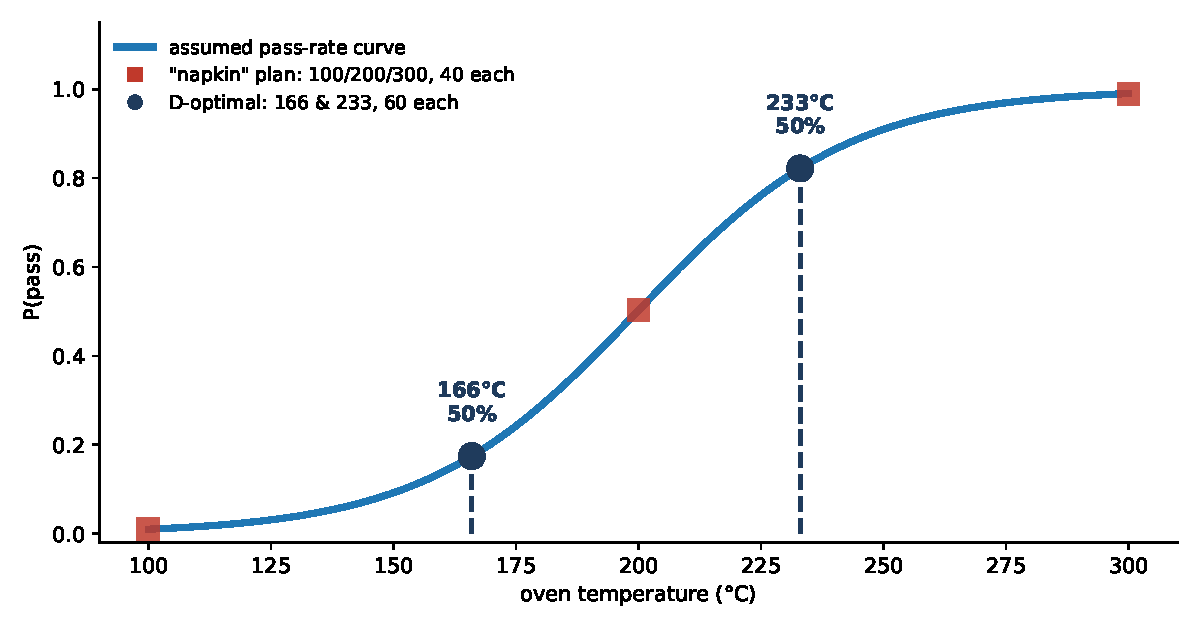
\includegraphics[width=\linewidth,height=0.7\textheight,keepaspectratio]{coating_design}
    \end{column}
    \begin{column}{0.48\textwidth}
      \small Pass/fail data follow a logistic curve
      \vspace{-0.3em}
      \[
        P(\text{pass}\mid x) = \frac{e^{\alpha+\beta x}}{1+e^{\alpha+\beta x}} .
      \]
      \vspace{-0.6em}
      \begin{itemize}
        \item The information a run carries now depends on $\theta=(\alpha,\beta)$:
              a piece tested where the curve is flat tells you almost nothing.
        \item So the optimal design depends on the unknown $\theta$: a \key{locally optimal design},
              built around a best guess (pilot data, expert opinion).
        \item Afterwards we check: how good is the design if the truth is different?
      \end{itemize}
    \end{column}
  \end{columns}
\end{frame}

\begin{frame}{The general problem, in one line}
  \[
    \xi^* \;=\; \arg\min_{\xi}\;
    \underbrace{\Phi_p}_{\text{criterion}}\Big(
      \underbrace{\Sigma\big(\xi,\;\overbrace{g(\theta)}^{\text{what we care about}}\big)}_{\text{variance of } \hat g \text{ under the model}}
    \Big),
    \qquad
    \xi=\{(x_i,w_i)\},\; x_i\in\underbrace{\mathcal X}_{\text{allowed settings}}
  \]
  \vspace{0.3em}
  \begin{itemize}
    \item \key{Criterion}: $D$, $A$, or any $\Phi_p$.
    \item \key{Parameters of interest}: all of $\theta$, a subset, or a function $g(\theta)$.
    \item \key{Model}: linear, logistic, Poisson, multinomial, ordinal, nonlinear regression, \ldots
    \item \key{Constraints}: the design region $\mathcal X$; possibly runs already made (multistage).
  \end{itemize}
  \vspace{0.3em}
  \begin{alertblock}{Two routes to a solution}
    \emph{Analytical}: elegant theorems, but case by case (one model, one criterion at a time).\;
    \emph{Algorithmic}: one method for everything---if it is fast and reliable. That is the rest of this talk.
  \end{alertblock}
\end{frame}

\begin{frame}{How do we know a design is optimal? One function to plot}
  \begin{columns}[c]
    \begin{column}{0.5\textwidth}
      \small For any candidate setting $x$, the \key{sensitivity function} $d(x,\xi)$ asks:
      \emph{how much would the criterion improve if a little of the budget moved to $x$?}
      \vspace{0.3em}
      \begin{block}{General equivalence theorem (Kiefer)}
        $\xi^*$ is optimal \;$\Longleftrightarrow$\; $d(x,\xi^*)\le 0$ for every $x\in\mathcal X$,
        with equality at the support points of $\xi^*$.
      \end{block}
      \begin{itemize}
        \item If $d(x,\xi)>0$ somewhere, adding that $x$ improves the design.
        \item For $D$-optimality: $d(x,\xi)=f(x)'M(\xi)^{-1}f(x)-k$.
      \end{itemize}
    \end{column}
    \begin{column}{0.5\textwidth}
      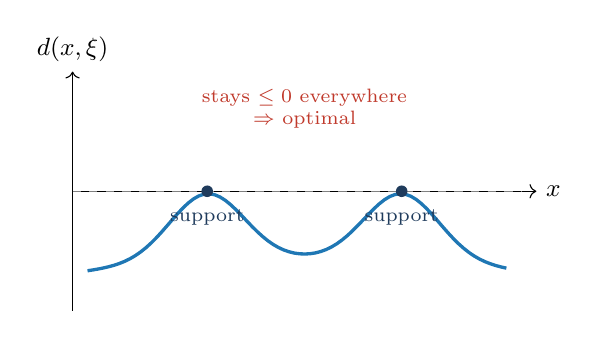
\begin{tikzpicture}[scale=0.95]
        \draw[->] (0,0) -- (6.2,0) node[right,font=\small] {$x$};
        \draw[->] (0,-1.6) -- (0,1.6) node[above,font=\small] {$d(x,\xi)$};
        \draw[gray,dashed] (0,0) -- (6,0);
        \draw[sky,very thick,domain=0.2:5.8,samples=80] plot (\x,{-0.9 + 0.9*exp(-((\x-1.8)^2)/0.5) + 0.9*exp(-((\x-4.4)^2)/0.5) - 0.02*(\x-3.1)^2});
        \fill[navy] (1.8,0) circle (2.2pt) node[below=3pt,font=\scriptsize,navy] {support};
        \fill[navy] (4.4,0) circle (2.2pt) node[below=3pt,font=\scriptsize,navy] {support};
        \node[font=\scriptsize,brick,align=center] at (3.1,1.1) {stays $\le 0$ everywhere\\ $\Rightarrow$ optimal};
      \end{tikzpicture}
    \end{column}
  \end{columns}
\end{frame}

% ============================================================================
\section{The OWEA algorithm}

\begin{frame}{What an algorithm must deliver}
  \begin{columns}[T]
    \begin{column}{0.5\textwidth}
      \begin{block}{Wish list}
        \begin{itemize}
          \item Any criterion: $D$, $A$, $\Phi_p$, \ldots
          \item Any parameters of interest: all, a subset, a function $g(\theta)$
          \item Any model: linear, GLM, nonlinear
          \item One-stage \emph{and} multistage (add to an existing experiment)
          \item Fast enough for large candidate sets and many factors
        \end{itemize}
      \end{block}
    \end{column}
    \begin{column}{0.5\textwidth}
      \begin{alertblock}{The obstacle}
        Classical algorithms nudge the weights a little at a time, insisting that the criterion improves
        at every step (``monotone'' updates). Safe, but slow---and the closed-form update rules only exist for special cases.
      \end{alertblock}
      \vspace{0.5em}
      \key{OWEA's idea:} stop nudging. For a \emph{given} set of support points, the optimal weights are the solution of a
      small system of equations---so \emph{solve} it.
    \end{column}
  \end{columns}
  \vspace{0.4em}
  \footnotesize Yang, Biedermann \& Tang (2013), \emph{JASA}: ``On optimal designs for nonlinear models: a general and efficient algorithm.''
\end{frame}

\begin{frame}{OWEA: two easy sub-problems, alternated}
  \small
  \begin{columns}[T]
    \begin{column}{0.48\textwidth}
      \begin{block}{1. Given the points, find the weights}
        With support $S=\{x_1,\ldots,x_k\}$ fixed, $\Phi_p(M(\xi))$ is a smooth function of the weights.
        Its minimum sits where
        \[
          \frac{\partial \Phi_p}{\partial w_i} = 0 \quad\text{or}\quad w_i = 0 .
        \]
        \key{Newton--Raphson} solves this in a handful of steps. Points whose weight hits $0$ are dropped.
      \end{block}
    \end{column}
    \begin{column}{0.48\textwidth}
      \begin{block}{2. Given the weights, find the next point}
        Compute the sensitivity function $d(x,\xi)$ on the candidate grid $\mathcal X$.
        \[
          x_{\max} = \arg\max_{x\in\mathcal X} d(x,\xi).
        \]
        If $d(x_{\max},\xi)\le\varepsilon$: \key{done, and certified optimal.}\\
        Otherwise \key{exchange}: add $x_{\max}$ to the support and go back to step 1.
      \end{block}
    \end{column}
  \end{columns}
  \vspace{0.3em}
  \centering
  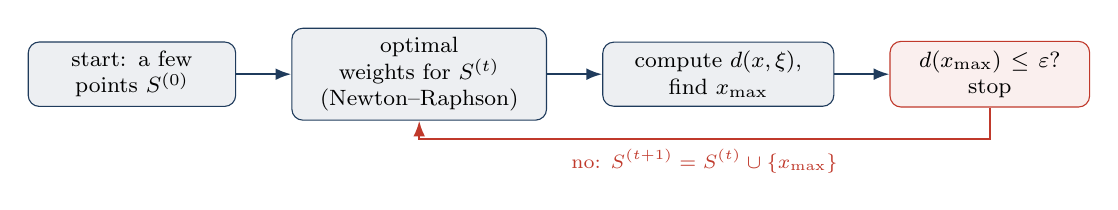
\begin{tikzpicture}[node distance=7mm, every node/.style={font=\footnotesize}]
    \node[draw=navy,rounded corners,fill=navy!8,text width=24mm,align=center,minimum height=8mm] (s) {start: a few points $S^{(0)}$};
    \node[draw=navy,rounded corners,fill=navy!8,text width=30mm,align=center,minimum height=8mm,right=of s] (w) {optimal weights for $S^{(t)}$\\(Newton--Raphson)};
    \node[draw=navy,rounded corners,fill=navy!8,text width=27mm,align=center,minimum height=8mm,right=of w] (d) {compute $d(x,\xi)$,\\ find $x_{\max}$};
    \node[draw=brick,rounded corners,fill=brick!8,text width=23mm,align=center,minimum height=8mm,right=of d] (e) {$d(x_{\max})\le\varepsilon$?\\ stop};
    \draw[-{Latex[length=2mm]},thick,navy] (s) -- (w);
    \draw[-{Latex[length=2mm]},thick,navy] (w) -- (d);
    \draw[-{Latex[length=2mm]},thick,navy] (d) -- (e);
    \draw[-{Latex[length=2mm]},thick,brick] (e.south) |- ++(0,-4mm) -| node[pos=0.25,below,font=\scriptsize,brick] {no: $S^{(t+1)}=S^{(t)}\cup\{x_{\max}\}$} (w.south);
  \end{tikzpicture}
\end{frame}

\begin{frame}{Why it is fast, and why it is general}
  \begin{itemize}\setlength{\itemsep}{0.7em}
    \item \key{Exact weights every round.} The weights are solved for, not nudged, so there is no slow creep towards the optimum;
          points whose weight reaches zero are dropped at once, and the support stays small.
    \item \key{The criterion enters only through $\Phi_p$ and its derivative.} Swap $D$ for $A$, or all parameters for a subset or a
          function $g(\theta)$: the loop is unchanged.
    \item \key{Multistage for free.} Runs already made contribute a fixed information matrix $I_{\xi_0}$; the algorithm optimises
          only what is added to it.
    \item \key{Any model.} All that is needed is the information a single run at $x$ carries, $I(x,\theta)$.
    \item \key{A certificate at the end.} The stopping rule \emph{is} the equivalence theorem, so the output comes with proof of
          optimality on the candidate set.
  \end{itemize}
\end{frame}

% ============================================================================
\section{The \texttt{OWEAdesign} package and web app}

\begin{frame}{\texttt{OWEAdesign}: the algorithm as a tool}
  \small
  \begin{columns}[T]
    \begin{column}{0.5\textwidth}
      \begin{block}{R package}
        \begin{itemize}
          \item \texttt{optimal\_design()} -- approximate designs (OWEA)
          \item \texttt{exact\_design()} -- whole-number allocations for $n$ runs
          \item \texttt{verify\_optimality()} -- check any design
          \item \texttt{compound\_design()} -- one design serving several objectives
          \item \texttt{simulate\_design()} -- see the gain by simulation
        \end{itemize}
        {\scriptsize\texttt{remotes::install\_github("minyangstat-eng/OWEAdesign")}}
      \end{block}
    \end{column}
    \begin{column}{0.5\textwidth}
      \begin{alertblock}{Web app -- no R, no installation}
        \centering {\footnotesize\url{https://statlab.math.uic.edu/OWEAdesign/}}\\[4pt]
        \raggedright
        A step-by-step wizard: describe the model, give a best guess, choose the criterion, click \emph{Compute}.
        Verify, simulate, download.
      \end{alertblock}
      \begin{itemize}
        \item Models: linear, logistic, Poisson, multinomial, ordinal
        \item Continuous and discrete factors, several at once
        \item Multistage: start from a pilot design or data set
      \end{itemize}
    \end{column}
  \end{columns}
\end{frame}

\begin{frame}{A real design problem: curing a coating}
  \small
  \begin{columns}[T]
    \begin{column}{0.56\textwidth}
      \begin{block}{The experiment}
        \begin{itemize}
          \item A protective coating on metal test pieces is \key{cured in an oven}; too cool and it stays soft.
                Each piece is scratch-tested and recorded as \key{pass or fail} (a binary response).
          \item The one factor we control: \key{oven temperature}, anywhere from 100 to 300\,$^\circ$C.
          \item Budget: \key{120 test pieces}, each cured at one temperature.
        \end{itemize}
        \vspace{-0.3em}
      \end{block}
      \begin{alertblock}{Goal}
        Estimate the whole pass-rate curve ($\alpha$ and $\beta$ in the logistic model) precisely,
        so that a safe operating temperature can be chosen later.
      \end{alertblock}
    \end{column}
    \begin{column}{0.42\textwidth}
      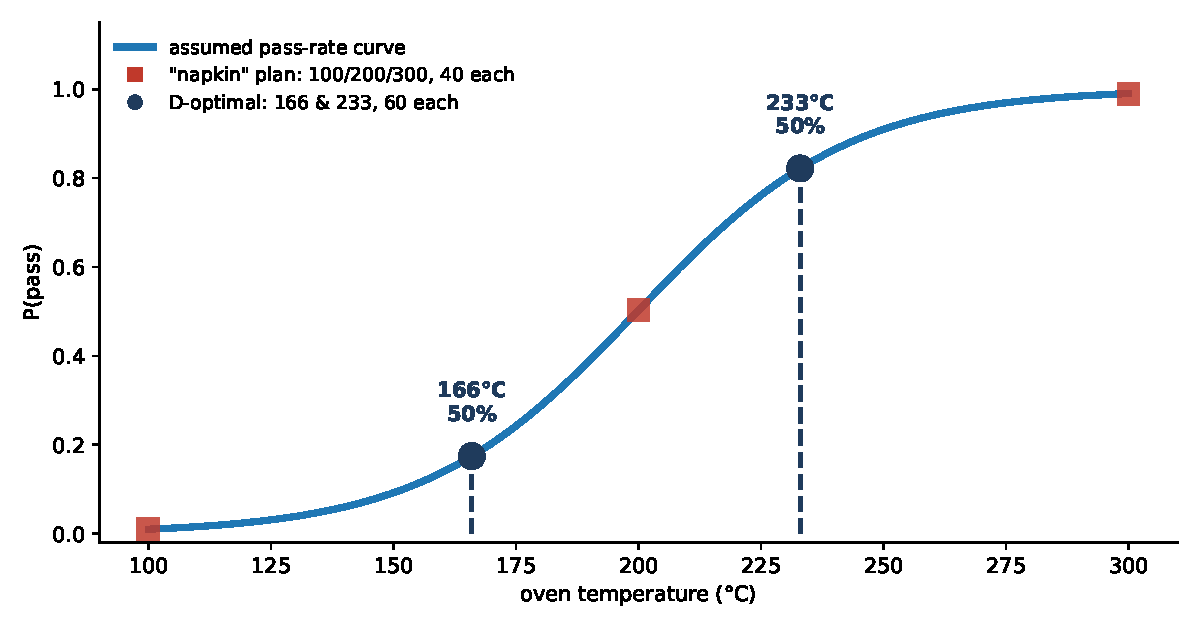
\includegraphics[width=\linewidth,height=0.36\textheight,keepaspectratio]{coating_design}
      \begin{block}{Prior knowledge, and the napkin plan}
        Bench experience: almost nothing passes at 100$^\circ$, almost everything at 300$^\circ$.\\[2pt]
        Natural plan: 100 / 200 / 300\,$^\circ$C, 40 pieces each. \hl{Is that good?}
      \end{block}
    \end{column}
  \end{columns}
\end{frame}

\begin{frame}{Step 1 -- what kind of problem, and which model}
  \begin{columns}[c]
    \begin{column}{0.5\textwidth}
      \shot{app_1_mode_c}
    \end{column}
    \begin{column}{0.5\textwidth}
      \shot{app_2_model}
    \end{column}
  \end{columns}
  \vspace{0.5em}
  \begin{itemize}
    \item One model, one goal $\Rightarrow$ \emph{classical}. (The \emph{compound} branch handles several models at once.)
    \item Pass/fail $\Rightarrow$ \emph{Logistic (binary)}. One covariate, \texttt{temp}, from 100 to 300, searched on a coarse-then-fine
          grid (steps \texttt{10, 1}); a grid-free continuous search is the other option.
  \end{itemize}
\end{frame}

\begin{frame}{Step 2 -- the best guess, and what ``best'' means}
  \begin{columns}[c]
    \begin{column}{0.5\textwidth}
      \shot{app_4_theta_c}
    \end{column}
    \begin{column}{0.5\textwidth}
      \shot{app_5_criterion_c}
    \end{column}
  \end{columns}
  \vspace{0.5em}
  \begin{itemize}
    \item The guess: intercept $-9.19$, slope $0.046$ (pass rate $\approx 1\%$ at 100$^\circ$, $\approx 99\%$ at 300$^\circ$). With pilot data the app fits these for you.
    \item Criterion: $D$-optimal, all parameters -- ``the most precise picture of the whole curve.''
  \end{itemize}
\end{frame}

\begin{frame}{Step 3 -- compute}
  \begin{columns}[c]
    \begin{column}{0.5\textwidth}
      \shot{app_8_result_table_c}
    \end{column}
    \begin{column}{0.5\textwidth}
      \shot{app_9_result_plot}
    \end{column}
  \end{columns}
  \vspace{0.5em}
  \begin{alertblock}{The answer}
    Two temperatures, \key{166$^\circ$ and 233$^\circ$C}, half the pieces at each. Not low--medium--high, not the extremes:
    two points on the steep part of the curve, where each piece is most informative. Certified optimal (max sensitivity $\approx 0$).
  \end{alertblock}
\end{frame}

\begin{frame}{Step 4 -- score the napkin plan}
  \begin{columns}[c]
    \begin{column}{0.5\textwidth}
      \shot{app_10_verify_c}
    \end{column}
    \begin{column}{0.5\textwidth}
      \small Paste any design into \emph{Verify optimality}. For the napkin plan (100/200/300, equal weights):
      \vspace{-0.4em}
      \begin{align*}
        \text{criterion (napkin)} &= -0.888\\
        \text{criterion (optimal)} &= -1.582\\
        \text{gap} &= 0.694 = \log 2
      \end{align*}
      \begin{alertblock}{Meaning}
        The napkin plan is \hl{50\% efficient}: 120 pieces on it are worth 60 on the optimal design.
        To match the optimal design's precision it would need \hl{240 pieces}.
        (The app also prints a guaranteed lower bound on the efficiency, here 47\%.)
      \end{alertblock}
      That is the fruit table again---in a real experiment.
    \end{column}
  \end{columns}
\end{frame}

\begin{frame}{How bad can a reasonable-looking plan be?}
  \centering
  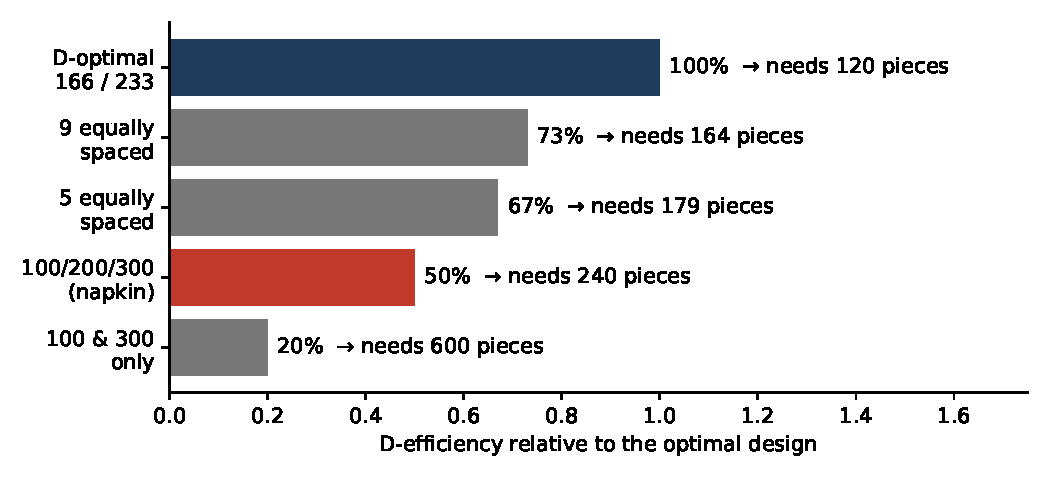
\includegraphics[width=0.8\linewidth]{efficiency}
  \vspace{-0.2em}
  {\footnotesize $D$-efficiency of common ``sensible'' allocations of 120 pieces, under the assumed curve.
  Spreading pieces across the flat parts of the curve is what costs information.}
\end{frame}

\begin{frame}{Step 5 -- make it real: an exact design for 120 pieces}
  \begin{columns}[c]
    \begin{column}{0.5\textwidth}
      \shot{app_11_exact_c}
    \end{column}
    \begin{column}{0.5\textwidth}
      \begin{itemize}
        \item Switch \emph{Design type} to \emph{Exact (integer runs)}, set $n=120$, recompute.
        \item Result: \key{60 pieces at 166$^\circ$, 60 at 233$^\circ$}.
        \item Download as CSV and hand it to the lab.
      \end{itemize}
      \vspace{0.6em}
      \begin{block}{Two flavours of the same design}
        \emph{Approximate}: fractions of the budget (theory, verification).\\
        \emph{Exact}: whole runs (what you actually do).
      \end{block}
    \end{column}
  \end{columns}
\end{frame}

\begin{frame}{Step 6 -- don't trust a formula: simulate}
  \begin{columns}[c]
    \begin{column}{0.55\textwidth}
      \shot{app_12_simulation_c}
    \end{column}
    \begin{column}{0.45\textwidth}
      \small The app simulates the experiment 1000 times from the assumed curve, fits the model each time and records the errors---for the
      optimal design and for any design you paste in.
      \begin{alertblock}{Result}
        Median squared error, napkin $\div$ optimal: \hl{$\approx 4\times$} for both parameters.
        The mean is far worse: with 40 pieces at 100$^\circ$C every piece fails, and those runs carry no information at all.
      \end{alertblock}
      Same 120 pieces, same cost, same model. Only the arrangement changed.
    \end{column}
  \end{columns}
\end{frame}

\begin{frame}{But my guess of the curve might be wrong}
  \small
  \begin{columns}[T]
    \begin{column}{0.5\textwidth}
      \begin{block}{Change the guess and recompute}
        Suppose the truth is milder: 3\% at 100$^\circ$, 97\% at 300$^\circ$.\\[3pt]
        New optimal design: $\{155^\circ, 244^\circ\}$, equal weights.\\
        The design moves a little, but keeps its shape: two points, equal weights.
      \end{block}
    \end{column}
    \begin{column}{0.5\textwidth}
      \begin{alertblock}{Score the plan we already had}
        Verify $\{166^\circ, 233^\circ\}$ under the new truth:\\
        criterion gap $0.058$ $\Rightarrow$ \key{94\% efficient}.\\[3pt]
        The napkin plan never gets close.
      \end{alertblock}
    \end{column}
  \end{columns}
  \vspace{0.4em}
  \begin{itemize}
    \item A locally optimal design is usually \emph{robust} to moderate errors in the guess---and the app lets you check exactly how robust.
    \item If the \emph{model itself} is in doubt, the \emph{compound} branch finds one design that is efficient under several models at once
          --- that is the next demo.
    \item Ran a pilot already? Paste the data: the app fits the curve and designs the \emph{next} stage around what you have learned.
  \end{itemize}
\end{frame}

\begin{frame}{Demo 2 -- what if the model itself is in doubt?}
  \small
  \begin{columns}[T]
    \begin{column}{0.5\textwidth}
      \begin{block}{Two beliefs on the bench}
        \begin{itemize}
          \item \key{Model 1: straight logistic.} Hotter is better, all the way to 300$^\circ$.
          \item \key{Model 2: logistic with a quadratic term.} Over-curing hurts: the pass rate peaks around 230$^\circ$ and
                falls again at 300$^\circ$.
        \end{itemize}
        Same experiment, same 120 pieces, same design region. Which design should we run?
      \end{block}
    \end{column}
    \begin{column}{0.5\textwidth}
      \begin{alertblock}{Each specialist is a gamble}
        \centering
        \begin{tabular}{lcc}\toprule
          efficiency under $\to$        & Model 1 & Model 2 \\ \midrule
          design optimal for Model 1     & 1.00 & \hl{0.17}$^*$ \\
          design optimal for Model 2     & \hl{0.47} & 1.00 \\ \bottomrule
        \end{tabular}\\[3pt]
        \raggedright\footnotesize $^*$essentially useless: two support points cannot estimate three parameters.
      \end{alertblock}
      A design that is perfect if you guessed the model right, and a disaster if you did not.
      \key{Compound design}: ask for one design that does well under \emph{both}.
    \end{column}
  \end{columns}
\end{frame}

\begin{frame}{Demo 2 -- setting it up in the app}
  \begin{columns}[c]
    \begin{column}{0.5\textwidth}
      \shotsm{cmp_3_objectives_c}
    \end{column}
    \begin{column}{0.5\textwidth}
      \shotsm{cmp_4_options_c}
    \end{column}
  \end{columns}
  \vspace{0.4em}
  \small
  \begin{itemize}
    \item Choose \emph{Several criteria at once (compound)}; the covariate and its range are shared by all objectives.
    \item Objective 1: logistic, $D$-optimal, the best guess from before. Objective 2: logistic with \emph{Quadratic terms} ticked,
          $D$-optimal, its own guess. Weights 1 and 1, applied to \emph{efficiencies}: care equally about each model's closeness to its own optimum.
  \end{itemize}
\end{frame}

\begin{frame}{Demo 2 -- one design that serves both models}
  \begin{columns}[c]
    \begin{column}{0.46\textwidth}
      \shotsm{cmp_6_design_c}
    \end{column}
    \begin{column}{0.54\textwidth}
      \shotsm{cmp_7_efficiency_c}
    \end{column}
  \end{columns}
  \vspace{0.3em}
  \small
  \begin{alertblock}{Reading the result}
    Four temperatures ($\approx$135, 171, 226, 300$^\circ$C) with weights 0.27, 0.24, 0.26, 0.22.
    Under Model 1 it is \key{77\%} efficient, under Model 2 \key{87\%}; the average, 0.82, is certified to be the
    best any single design can do. That 18\% shortfall is the price of insurance against picking the wrong model
    --- versus losing 53\% or 83\% by betting on one specialist.
  \end{alertblock}
\end{frame}

\begin{frame}{Demo 2 -- the three designs side by side}
  \centering
  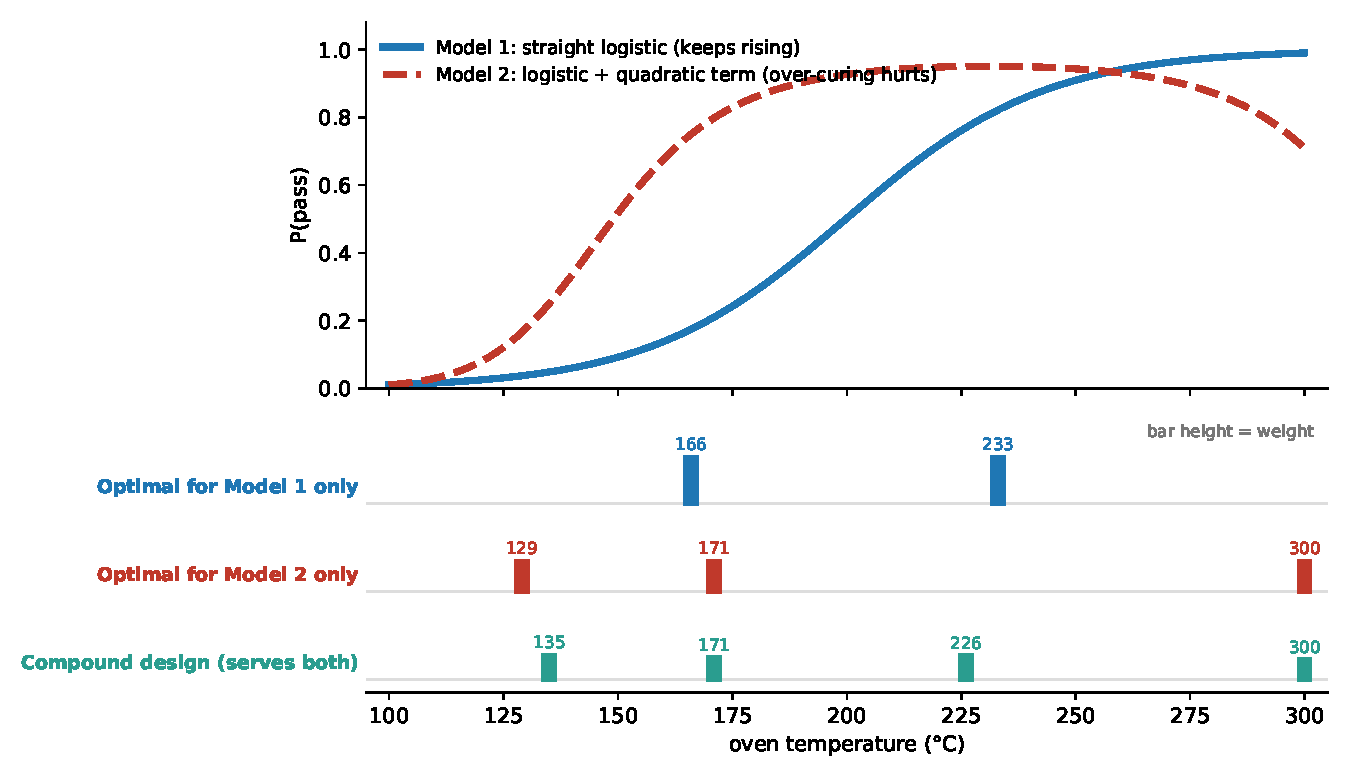
\includegraphics[width=\linewidth,height=0.72\textheight,keepaspectratio]{compound_designs}
  \vspace{-0.3em}
  {\footnotesize The compound design keeps the two ``steep-part'' points of Model 1 and adds the end point and a low point that
  Model 2 needs to detect the bend. Any design you prefer can be pasted into \emph{Score another design} and rated on the same scale.}
\end{frame}

\begin{frame}[fragile]{The same thing in R}
\begin{lstlisting}
library(OWEAdesign)

# information vector f(x, theta) for a logistic model with one covariate
info_vec <- function(x, theta) {
  q <- c(1, x); eta <- sum(q * theta)
  (exp(eta / 2) / (1 + exp(eta))) * q
}

res <- optimal_design(info_vector   = info_vec,
                      theta         = c(-9.19, 0.046),   # best guess
                      design_box    = list(c(100, 300)), # allowed temperatures
                      step_sequence = c(10, 1),          # coarse -> fine grid
                      p             = 0)                 # 0 = D-optimal, 1 = A-optimal

cbind(temp = res$support, weight = res$weights)
#>   temp weight
#>    166    0.5
#>    233    0.5
\end{lstlisting}
\vspace{-0.3em}
{\footnotesize Everything the app does is one function call away: \texttt{exact\_design()}, \texttt{verify\_optimality()}, \texttt{compound\_design()}, \texttt{simulate\_design()}.}
\end{frame}

% ============================================================================
\section{Take-home}

\begin{frame}{Take-home messages}
  \begin{enumerate}
    \item \key{Design is where information is created.} The same budget, arranged well, can be worth two or four times as much.
    \item \key{Optimal design has a precise meaning:} choose the settings and their shares so a chosen criterion of the
          information matrix is best---and one function, $d(x,\xi)$, certifies that you got there.
    \item \key{OWEA} turns the theory into a general, fast procedure: solve for the weights, add the most valuable point, repeat.
    \item \key{You do not need to be a statistician to use it.} Describe the experiment in the web app, click \emph{Compute},
          verify, simulate, download --- and when the model is uncertain, ask for a compound design.
  \end{enumerate}
  \vspace{0.8em}
  \begin{alertblock}{Next time you plan an experiment}
    Before you settle for low--medium--high, spend five minutes at \url{https://statlab.math.uic.edu/OWEAdesign/}.
  \end{alertblock}
\end{frame}

\begin{frame}{Key reference and links}
  \begin{block}{Key reference}
    Yang, M., Biedermann, S., and Tang, E. (2013). On optimal designs for nonlinear models: a general and efficient algorithm.
    \emph{Journal of the American Statistical Association}, 108, 1411--1420.
  \end{block}
  \vspace{1em}
  \begin{columns}[T]
    \begin{column}{0.5\textwidth}
      \key{R package}\\ {\footnotesize\url{https://github.com/minyangstat-eng/OWEAdesign}}\\[3pt]
      {\scriptsize\texttt{remotes::install\_github("minyangstat-eng/OWEAdesign")}}
    \end{column}
    \begin{column}{0.5\textwidth}
      \key{Web app (no installation)}\\ {\footnotesize\url{https://statlab.math.uic.edu/OWEAdesign/}}
    \end{column}
  \end{columns}
  \vspace{1.2em}
  {\small Supported by the National Science Foundation.}
  % TODO: add the NSF grant number(s) you wish to acknowledge.
\end{frame}

\begin{frame}[standout]
  Thank you.\\[0.5em]
  {\normalsize Questions? \qquad \texttt{myang2@uic.edu}}
\end{frame}

\end{document}
